\documentclass[fleqn]{article}
\usepackage{amsmath}
\usepackage[dvips]{graphicx}
\bibliographystyle{plain}
%__________________________________
\begin{document}

\section*{\center Taylor Impact Test}
\subsection*{\underline{Problem Description}}
This is a simulation of an Taylor impact experiment calculation from 
\cite{Gust82} in a copper cylinder at 718 K that is fired at a
rigid anvil at 188 m/s.  The copper cylinder has a length of 30 mm and
a diameter of 6 mm.  The cylinder rebounds from the anvil after 100 $\mu$s.
 
\subsection*{\underline{Simulation Specifics}}
\begin{description} 
\item [Component used:] \hfill MPM
\item [Input file name:] \hfill taylorImpact.ups
\item [Command used to run input file:]\hfill sus taylorImpact.ups
\item [Simulation Domain:]\hfill 8 mm x 33 mm x 8 mm

\item [Cell Spacing:]\hfill \\ 
  1/3 mm x 1/3 mm x 1/3 mm (Level 0)

\item [Example Runtimes:] \hfill \\
 1 hour 20 min.   (1 processor, AMD Opteron 2.2 GHz)\\

\item [Physical time simulated:] \hfill 100 $\mu$seconds

\item [Associate scirun network:] \hfill taylorImpact.srn

\end{description}

\section*{\underline{Results}}

Figure~\ref{fig:taylorImpact} shows a snapshot of the simulation after the
cylinder begins to rebound.
\begin{figure}[b]
  \center
%  \scalebox{0.2}{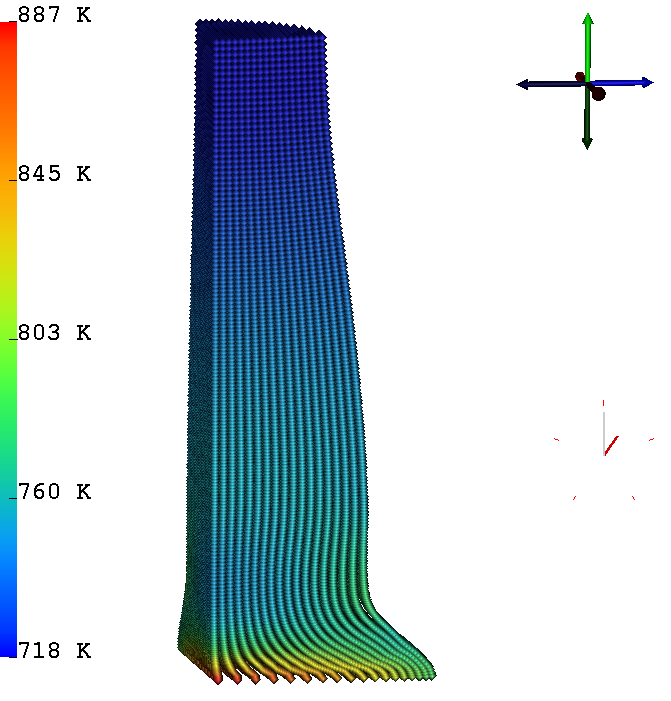
\includegraphics{taylorImpact.png}}
  \caption{Taylor impact simulation.  Particles colored according to
           temperature.}
  \label{fig:taylorImpact}
\end{figure}

Additional data are available within the uda in the form of "dat" files.

\bibliography{../references}

\end{document}
